\documentclass[a4paper, 10pt]{article}

\usepackage{hyperref}
\usepackage[utf8]{inputenc}
\usepackage[french]{babel}
\usepackage{eurosym} % \oe{} ...
\usepackage{graphicx}
\usepackage[T1]{fontenc}
\usepackage{geometry}
\usepackage{fancyhdr}
\usepackage{lastpage}
\usepackage{paralist}
\usepackage{listings}
\usepackage{color}

\lstset{language=Python, frame=shadowbox, rulesepcolor=\color{black}}

\geometry{hmargin=1.5cm, vmargin=2cm }
\pagestyle{fancy}
\setlength\parindent{0pt}

\lhead{IMT Lille Douai -- UV MAD} \lfoot{G.L.}
\rhead{TD/TP 02 - Décisions sous incertitude}
\rfoot{Page : \thepage/\pageref{LastPage}}
\cfoot{} \chead{}

\begin{document}
\author{IMT Lille Douai -- UV-MAD}
\date{}
\title{\Large{\textbf{TD/TP 02 - Décisions sous incertitude \\ Exprimer et calculer des statistiques corrélées}}}
\maketitle
\thispagestyle{fancy}

\section*{Nom(s) et prénom(s): \_\_\_\_\_\_\_\_\_\_\_\_\_\_ $\quad$ \_\_\_\_\_\_\_\_\_\_\_\_\_\_}

\bigskip

\section{Probabilité de mourir}

  On souhaite réaliser une intelligence artificielle (\emph{IA}) basée sur la probabilité que l'on a de mourir si on continue à jouer.
  Dans un premier temps on travaille dans un cadre simplifié où on ne lancera qu'un dé à chaque tour.

\begin{itemize}[$\bigcirc$]
  \item Configurer le jeu pour ne jouer qu'avec un seul dé.
  Dans la fonction \emph{main} de la classe \emph{ZombieDice}, le premier paramètre de la fonction \emph{singleGame} représente le nombre de dés utilisés dans le jeu.
%   \item Générer une nouvelle classe de personnage non joueur (\emph{npc}) nommé \emph{WillDie0}.
%   Implémenter dans \emph{WillDie0} un calcul de la probabilité de mourir si le type du dé à lancer est connu.
%   Utiliser cette information pour adapter son choix de jouer ou non.
  \item De quelles variables du jeu dépend la probabilité de mourir ?
  \medskip

\_\_\_\_\_\_\_\_\_\_\_\_\_\_\_\_\_\_\_\_\_\_\_\_\_\_\_\_\_\_\_\_\_\_\_\_\_\_\_\_\_\_\_\_\_\_\_\_\_\_\_\_\_\_\_\_\_\_\_\_\_\_

  \medskip

\_\_\_\_\_\_\_\_\_\_\_\_\_\_\_\_\_\_\_\_\_\_\_\_\_\_\_\_\_\_\_\_\_\_\_\_\_\_\_\_\_\_\_\_\_\_\_\_\_\_\_\_\_\_\_\_\_\_\_\_\_\_

  \medskip

\end{itemize}



\section{Comprendre les réseaux bayésiens}


  Les réseaux bayésiens permettent de représenter schématiquement les liens de causalité.
  Un n\oe{}ud représente une variable un arc orienté modélise une dépendance statistique sur l'affectation de valeurs (la variable du n\oe{}ud parent influence les valeurs pour la variable du n\oe{}ud fils).

  \url{https://fr.wikipedia.org/wiki/R\%C3\%A9seau_bay\%C3\%A9sien} (fr)

  \begin{minipage}{0.64\textwidth}

  \medskip
  Par exemple dans Zombie Dice, les probabilités que le zombie attrape l'humain (Brain) que celui-ci s'échappe (Run) ou se défende (Shot) dépendent du type de dés (Easy, Medium ou Hard) en main.

  \medskip
  Pour chaque n\oe{}ud (A, B et C dans l'exemple ci-contre), on établit alors un tableau reprenant les probabilités d'affectation de la variable.
  Dans la mesure où il y a une ou plusieurs dépendances (n\oe{}ud A dans l'exemple), ces probabilités sont exprimées en fonction des valeurs sur les variables dont elle dépend.
  Dans l'exemple, A et C peuvent valoir 0 ou 1 et B 0, 1 ou 2. Si B vaux 1 (avec une probabilité donc de $0.4$) et C vaux 0 alors il y a une probabilité de $0.8$ que A vaille 0 et de $0.2$ qu'il vaille 1.

  \end{minipage}
  \begin{minipage}{0.33\textwidth}

     \centering
     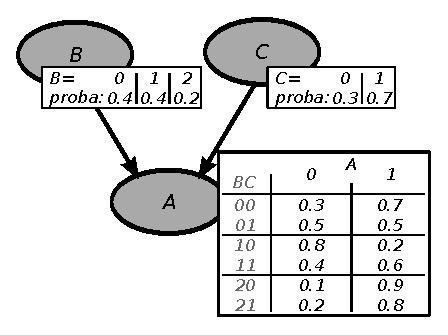
\includegraphics[width=0.99\textwidth]{fig/resbay}

  \end{minipage}


\begin{itemize}[$\bigcirc$]
  \item

  \begin{minipage}{0.4\textwidth}

  Compléter le tableau lié au lancer d'un dé (un dé indéfini n'affecte pas le jeu, on a donc une probabilité certaine d'avoir un \emph{run}):

  \end{minipage}
  \begin{minipage}{0.02\textwidth}

  \end{minipage}
  \begin{minipage}{0.5\textwidth}

     \centering

	  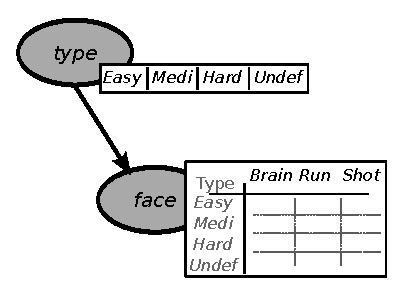
\includegraphics[width=0.99\textwidth]{fig/resbay_ZD1}

  \end{minipage}

  \item La probabilité de mourir découle directement de la face du dé lancé et du nombre de balles déjà encaissées.
  Reprendre et compléter le réseau bayésien précédent pour faire apparaître la probabilité de mourir ``dead'' (Listing~1).

  \item Compléter le réseau bayésien précédent pour exprimer aussi les probabilités sur le type du dé lancé  (Listing~1).

\begin{lstlisting}[caption={Reseau bayésien mourir avec un dé}]

























.
\end{lstlisting}

  \item Le tableau associé au n\oe{}ud \emph{type} est de quelle dimension ?

  \medskip

  \_\_\_\_\_\_\_\_\_\_\_\_\_\_\_\_\_\_\_\_\_\_\_\_\_\_\_\_\_\_\_\_\_\_\_\_\_\_\_\_\_\_\_\_\_\_\_\_\_\_\_\_\_\_\_\_\_\_\_\_\_\_

%   \item En quoi le N\oe{}ud ``\emph{dead}'' est-il particulier dans ce réseau ?
%   \medskip
% \_\_\_\_\_\_\_\_\_\_\_\_\_\_\_\_\_\_\_\_\_\_\_\_\_\_\_\_\_\_\_\_\_\_\_\_\_\_\_\_\_\_\_\_\_\_\_\_\_\_\_\_\_\_\_\_\_\_\_\_\_\_

%
%   \medskip

  \end{itemize}

  \section{Implémentation simple}

  Dans le cadre du \emph{TP} sur \emph{ZombieDice} il vous est proposé une implémentation simple de réseaux bayésiens.
  Cependant il existe de nombreuses librairies vous proposant des implémentations plus complètes, citons notamment \emph{Weka} pour le langage JAVA :
  \begin{itemize}
    \item \url{http://weka.wikispaces.com/}
    \item \url{http://www.cs.waikato.ac.nz/~remco/weka_bn/}
  \end{itemize}
  ou \emph{BayesPy} en python et l'ensembles des projets similaires qu'ils citent:
  \begin{itemize}
    \item \url{https://www.bayespy.org/intro.html}
  \end{itemize}

  Restons simple donc, l’outil proposé se base sur une classe \emph{BayesianVariable} disponible dans le package \emph{décision}.
  Cette classe représente des n\oe{}uds conditionnels.
  Dans ce cas un attribut \emph{parent} liste l'ensemble des variables (classe \emph{DiscreteVariable} ou héritiés) dont dépend la variable représentée par le n\oe{}ud
  une méthode \emph{distribution} retourne les probabilités conditionnelles sous forme d'un dictionnaire.
  Un état conditionnel est une affectation des variables parents.

  \begin{itemize}[$\bigcirc$]
    \item regarder les classes \emph{DiscreteVariable} et \emph{BayesianVariable} ainsi que le script \emph{test-bayesian.py} pour comprendre le fonctionnement (cf. nouvelle version sur bitbucket).
    \item creer un réseau Bayesien permettant de calculer la probabilité de mourir tel que vous l'avez défini précédemment.
    \item les méthodes \emph{dotnode} et \emph{dotgraph} de la classe \emph{BayesianVariable} permet de générer le graph dans le format \emph{dot\footnote{\url{https://en.wikipedia.org/wiki/DOT\_(graph\_description\_language)}}}. Générez un \emph{graph} et visualisez-le via : \url{http://rise4fun.com/agl}.
    \item creer une fonction permettant de visualiser tout les n\oe{}uds.
  \end{itemize}

\section{Calcul de probabilités corrélées}

  Les réseaux bayésiens offrent avec une représentation schématique, un cadre de travail pour calculer les probabilités inférées (résultant de dépendances de causalité).

  Les probabilités d'affectation d'une variable $A$ sont calculées en sommant le produit des probabilités liées aux variables dont elle dépend.
  Les probabilités d'affectation peuvent donc être calculé sur la base du tableau du n\oe{}ud dans le réseau bayésien et d'une distribution de probabilités sur les variables cause.

  \begin{center}
    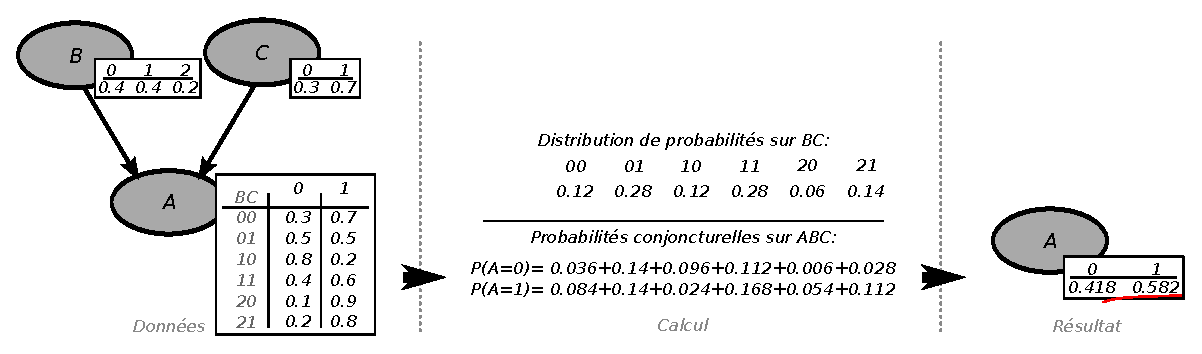
\includegraphics[width=0.8\textwidth]{fig/resbay_calcul}
  \end{center}

\begin{itemize}[$\bigcirc$]
    \item Selon cette logique et en s'appuyant sur le réseau proposé, quelles sont les probabilités sur la face au lancer et la probabilité de mourir avec la distribution de probabilités suivante:

    $\mathit{type}= \{P(\mathit{EASY})= 0.4,\ P(\mathit{MEDIUM})= 0.4,\ P(\mathit{HARD})= 0.2,\ P(\mathit{UNDEF})= 0.0\}$

    et $\mathit{shot}= \{P(1)= 0.3,\ P(2)= 0.7\}$.

\medskip

\_\_\_\_\_\_\_\_\_\_\_\_\_\_\_\_\_\_\_\_\_\_\_\_\_\_\_\_\_\_\_\_\_\_\_\_\_\_\_\_\_\_\_\_\_\_\_\_\_\_\_\_\_\_\_\_\_\_\_\_\_\_

\medskip

\_\_\_\_\_\_\_\_\_\_\_\_\_\_\_\_\_\_\_\_\_\_\_\_\_\_\_\_\_\_\_\_\_\_\_\_\_\_\_\_\_\_\_\_\_\_\_\_\_\_\_\_\_\_\_\_\_\_\_\_\_\_

\medskip

\_\_\_\_\_\_\_\_\_\_\_\_\_\_\_\_\_\_\_\_\_\_\_\_\_\_\_\_\_\_\_\_\_\_\_\_\_\_\_\_\_\_\_\_\_\_\_\_\_\_\_\_\_\_\_\_\_\_\_\_\_\_

\medskip
    \item Les méthodes \emph{setOn} et \emph{setAt} permettent d'affecter une valeur $v$ à une variable $x$ ($P(x=v)= 1$. L'appel à la méthode \emph{update} permet d'actualiser les probabilités d'une variable en s'appuyant sur les probabilités des parents.
    À l'aide de ces deux méthodes, calculez la probabilité de mourir en jouant encore un coup et servez-vous-en dans une nouvelle IA, pour déterminer l'action à faire.

    \item Tester votre IA en tournois.
\end{itemize}

  \section{Espérance de gain et réseaux bayésiens dynamiques}

  L'idée est de ne plus se limiter à la probabilité de mourir ou non en continuant de jouer, mais de confronter cette probabilité à l'espérance que l'on peut avoir d'engranger plus de gain (de cerveaux dans ZombieDice).

  Idéalement dans le jeu, il nous faudrait exprimer l'évolution possible du nombre de cerveaux.
  Cependant le nombre de cerveaux dépend de la face tirée et de lui même (nombre de cerveaux déjà engrangés).

  \begin{itemize}[$\bigcirc$]
   \item Exprimer l'évolution du nombre de cerveaux dans le réseau bayésien précédent.
  \end{itemize}

  Dans le cadre d'un déroulement séquentiel pour la modélisation de systèmes évolutifs, on a besoin d'étendre la définition des réseaux bayésiens aux réseaux bayésiens dynamiques\footnote{\url{https://fr.wikipedia.org/wiki/R\%C3\%A9seau_bay\%C3\%A9sien_dynamique}}

  \begin{center}
    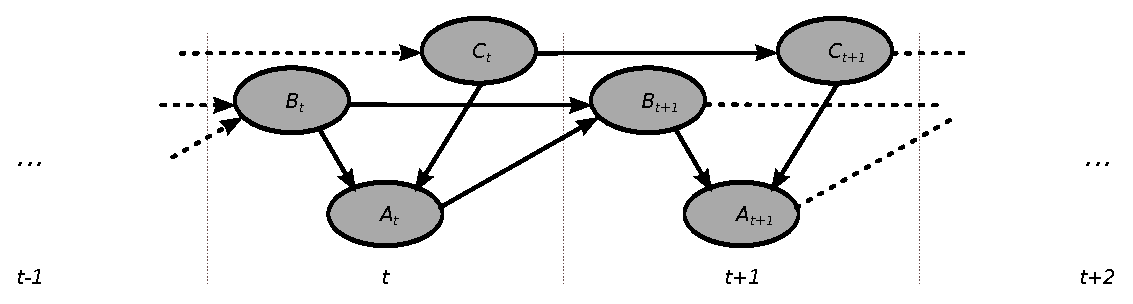
\includegraphics[width=0.8\textwidth]{fig/resbay_dyn}
  \end{center}

  \newpage

  L'idée alors, dans le réseau bayésien, consiste à dédoubler les variables dans le temps $t+1$ et représenter les dépendances entre les variables au temps $t$ et elle même au temps $t+1$. On exprime l'évolution du système à la manière de suites mathématiques

  \begin{itemize}[$\bigcirc$]
      \item Reprendre votre réseau en dédoublant les variables d'états (stock, main initiale, cerveaux et balles) pour le définir un modèle dynamique.

      \begin{lstlisting}[caption={Réseau bayésien dynamique}]

























.
\end{lstlisting}

    \item Implémenter ce nouveau réseau dans un nouveau \emph{npc} \emph{Horizon1}

    \item Le gain espéré de l'action de jouer exprime alors le produit du nombre de cerveaux que l'on mangerait par la probabilité que cela se produise.
    Soit à 1 dé:

    $V(\mathit{play})= \mathit{brain} \times P(\mathit{brain}_{t+1}= \mathit{brain}) + (\mathit{brain}+1) \times P(\mathit{brain}_{t+1}= \mathit{brain}+1)$

    Comparer le gain espéré en jouant avec le gain immédiat de scorer pour décider de continuer ou non.

     \item expérimenter en tournois votre nouvelle IA.

  \end{itemize}

  \section{Retour sur un jeu à 3 dés}

  La version à $3$ dé n'est finalement qu'une répétition du réseau bayésien proposé pour un dé.

\begin{itemize}[$\bigcirc$]
   \item Mettre en place une nouvelle IA pour prendre en compte une main de $3$ dés.
   \item Générer le ``\emph{dot}'' de votre réseau bayésien et tester votre IA.
  \end{itemize}

\end{document}
